\documentclass[10pt]{article}
\usepackage{amsmath, amsthm, amssymb}
\usepackage{graphicx}
\usepackage{caption}
\usepackage{subcaption}
\usepackage{url}
\usepackage{tikz}
\usetikzlibrary{calc,through}
\usepackage[latin1]{inputenc}
\newtheorem{theorem}{Theorem}

\usepackage[pdftex,bookmarks=true, pdftitle={Nobby Demo},
pdfauthor={Oliver Nagy}, colorlinks=true,
citecolor=black, linkcolor=black]{hyperref}

% Define font for vectors.
\newcommand{\mvec}[1]{\mathbf{#1}}

% Define a color.
\definecolor{blue}{rgb}{0,0.5,0.99}

% Meta tags (Nobby will extract them and put them as comments into the
% HTML file).
\title{Nobby Demo}
\author{Oliver Nagy (olitheolix@gmail.com)}

\begin{document}
\maketitle

\section{Section One}
\label{sec:one}
This file demonstrates some of the constructs Nobby can convert to
HTML. Nobby relies on properly formatted \LaTeX code to do its work
properly.

Here is Pythagoras' theorem in an \emph{align} environment:
\begin{align*}
  \label{eq:pyth}
  z = \sqrt{x^2 + y^2}.
\end{align*}
Here it is again as an inline formula: $z = \sqrt{x^2 + y^2}$.

That was it, except for a link to \hyperref[eq:pyth]{Pythagoras} and
another \hyperref[eq:rel]{famous formula}.

Nobby automatically escapes the <> characters. It is therefore safe to
write <strong> or </strong> without accidentally inserting HTML tags.

Similarly, Nobby also translate quotes: ``text in quotes'' and
escaped \LaTeX symbols like ``\$'', ``\{``, ``\}'' and ``\%'' to
proper HTML, ie. without the leading backslash.

\subsection{More formatting}
Reference to \hyperref[sec:one]{previous section}.

You can, of course, \emph{emphasise} something.

An embedded math symbol $x=1$ here, or a more elaborate formula:
$e^{i\pi} + 1 = 0$.

Here is some plain text. {{This sentence is actually an SVG image.}}

Three dots are sometimes useful\ldots as is the \texttt{typewriter
  font}.

This is a \textbf{bold} statement.

\subsection{Environments}
Nobby does not know about environments. Plugins compound this
problem. Nobby ships with some plugins to convert standard
environments.

\subsubsection{Itemize}
\begin{itemize}
\item Item 1
\item Item 2
\end{itemize}

\subsubsection{Enumerate}
\begin{enumerate}
\item Item 1
\item Item 2
\end{enumerate}

\subsubsection{Equation}
\begin{equation}
  \label{eq:rel}
  E = mc^2.
\end{equation}

\subsubsection{Theorem}
There is no default plugin for theorems. The entire theorem
environment will thus be an image.
\begin{theorem}
  This is a theorem.
\end{theorem}

Next is a comment. You cannot see it because it is, well, a
comment. To see it, switch to the source code in your browser.
% By the way, you are free to add comments. Comments will show up in
% the HTML file (as comments, obviously).

\section{Figures}
Here is a floating table. \LaTeX would put it at a visually pleasing
position, whereas Nobby put it right where it was defined.
\begin{table}
  \centering
  \begin{tabular}{c | c c c c}
    & $\frac{\pi}{6}$& $\frac{\pi}{4}$& $\frac{\pi}{2}$ & $\pi$\\[1mm]
    \hline
    \rule{0cm}{4mm}$\sin(\phi)$& $\frac{1}{2}$ & $\frac{1}{\sqrt{2}}$& $1$ & $0$\\
    \rule{0cm}{4mm}$\cos(\phi)$& $\frac{\sqrt{3}}{2}$ & $\frac{1}{\sqrt{2}}$& $0$&$-1$
  \end{tabular}
  \caption{Floating table}
\end{table}

A conventional figure environment that uses the
\texttt{\textbackslash{subcaption}} package. The code and figures for
the next example are actually from the
\href{http://en.wikibooks.org/wiki/LaTeX/Floats,_Figures_and_Captions}{Wikimedia}
on \LaTeX. Note that the image is a PNG (hence the coarser appearance)
because the inclusion of the three other images exceeds the image size
threshold (you can adjust it in Nobby's \texttt{config.py} file).\\


\begin{figure}
  \centering
  \begin{subfigure}[b]{0.3\textwidth}
    \includegraphics[width=\textwidth]{gull}
    \caption{A gull}
    \label{fig:gull}
  \end{subfigure}%
  ~ %add desired spacing between images, e. g. ~, \quad, \qquad etc.
  % (or a blank line to force the subfigure onto a new line)
  \begin{subfigure}[b]{0.3\textwidth}
    \includegraphics[width=\textwidth]{tiger}
    \caption{A tiger}
    \label{fig:tiger}
  \end{subfigure}
  ~ %add desired spacing between images, e. g. ~, \quad, \qquad etc.
  % (or a blank line to force the subfigure onto a new line)
  \begin{subfigure}[b]{0.3\textwidth}
    \includegraphics[width=\textwidth]{mouse}
    \caption{A mouse}
    \label{fig:mouse}
  \end{subfigure}
  \caption{Pictures of animals}\label{fig:animals}
\end{figure}

Reference to \hyperref[sec:one]{previous section}.

\section{TikZ Image}
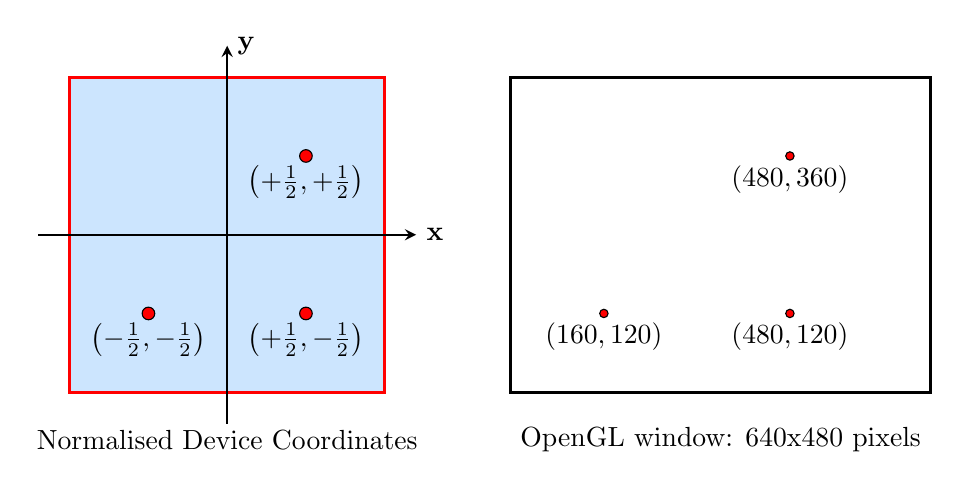
\begin{tikzpicture}[scale=2, >=stealth]
  \draw[very thick,fill=blue!20!white,draw=red] (-1,-1) rectangle (1,1);
  \node[] at(0,-1.3) {Normalised Device Coordinates};
  \node[right] at(1.8,-1.3) {OpenGL window: 640x480 pixels};

  \draw[thick,->] (-1.2,0) -- (1.2,0) node[right] {$\mvec{x}$};
  \draw[thick,->] (0,-1.2) -- (0,1.2) node[right] {$\mvec{y}$};

  \filldraw[fill=red,draw=black] (-.5,-.5) circle (0.04)
  node[below]{$\left(-\frac{1}{2},-\frac{1}{2}\right)$};

  \filldraw[fill=red,draw=black] (+.5,-.5) circle (0.04)
  node[below]{$\left(+\frac{1}{2},-\frac{1}{2}\right)$};

  \filldraw[fill=red,draw=black] (+.5,+.5) circle (0.04)
  node[below]{$\left(+\frac{1}{2},+\frac{1}{2}\right)$};

  \begin{scope}[scale=2/3,xshift=2.7cm,yshift=-1.5cm]
    \draw[very thick] (0,0) rectangle (4,3);

    \filldraw[fill=red,draw=black] (0.888, 0.75) circle (0.04)
    node[below]{$(160, 120)$};

    \filldraw[fill=red,draw=black] (2.66, 0.75) circle (0.04)
    node[below]{$(480, 120)$};

    \filldraw[fill=red,draw=black] (2.66, 2.25) circle (0.04)
    node[below]{$(480, 360)$};
  \end{scope}
\end{tikzpicture}

The end.
\end{document}
